\documentclass[a4paper,11pt]{article}
\usepackage{cmap}
\usepackage{polski}
\usepackage[T1]{fontenc}
\usepackage[utf8]{inputenc}
\usepackage{graphicx}
\usepackage{minted}
\usepackage{titlesec}

\titlelabel{\thetitle.\quad}

\date{
{Data zajęć: 24.01.2019\hfill Data oddania: 28.01.2019}
\\
{Termin zajęć: Pon. TP 9:15\hfill Prowadzący zajęcia: Mgr inż. Szymon Datko}
}
\title{Sprawozdanie nr 5}
\author{Jakub Majewski 238902}

\makeatletter
\renewcommand{\maketitle}{
   \begin{titlepage}
     \begin{center}
       {\@date}
       \\
       \par\vspace{3ex}
       {\LARGE\@title}
       \par\vspace{1ex}
       \begin{tabular}[t]{c}
         \@author
       \end{tabular}
     \end{center}
     \@thanks
   \end{titlepage}
}
\makeatother

\begin{document}

\begin{center}\Large
    Grafika Komputerowa i Komunikacja Człowiek-Komputer
\end{center}

\hrule
    {\let\newpage\relax\maketitle}
\hrule

% ******************************* OPIS TEMATU *******************************

\section{Opis tematu}

Temat: OpenGL - Teksturowanie powierzchni obiektów. \\ \\
Zrealizowane zadania: \\
1. nałożenie tekstury na pojedynczą płaszczyznę w krztałcie trójkąta, \\
2. oteksturowanie wielościanu, \\
3. oteksturowanie obiektu powstałego z powierzchni opisanej parametrycznie. \\

% ******************************* OPIS NAJWAŻNIEJSZYCH FRAGMENTÓW KODU *******************************

\newpage
\section{Opis najważniejszych fragmentów kodu}

\noindent 1. Metoda inicjalizująca możliwość teksturowania obiektów
\begin{minted}[linenos,tabsize=2,breaklines]{CPP}
void World::Init_Texturing() {

	//  Odczytanie danych o teksturze z pliku o formacie .tga
	pBytes = LoadTGAImage("res/test.tga", &ImWidth, &ImHeight, &ImComponents, &ImFormat);

	// Zdefiniowanie tekstury 2D 
	glTexImage2D(GL_TEXTURE_2D, 0, ImComponents, ImWidth, ImHeight, 0, ImFormat, GL_UNSIGNED_BYTE, pBytes);
	// Usunięcie z pamięci tablicy pBytes
	free(pBytes);

	// Włączenie mechanizmu i ustawienie trybu teksturowania
	glEnable(GL_TEXTURE_2D);
	glTexEnvi(GL_TEXTURE_ENV, GL_TEXTURE_ENV_MODE, GL_MODULATE);

	// Określenie sposobu nakładania tekstur
	glTexParameteri(GL_TEXTURE_2D, GL_TEXTURE_MIN_FILTER, GL_LINEAR);
	glTexParameteri(GL_TEXTURE_2D, GL_TEXTURE_MAG_FILTER, GL_LINEAR);
}
\end{minted}
\newpage

\noindent 2. Tworzenie instancji obiektu przechowującego nagłówek plików typu .tga
\begin{minted}[linenos,tabsize=2,breaklines]{CPP}
#pragma pack(1)            
typedef struct
{
	GLbyte    idlength;
	GLbyte    colormaptype;
	GLbyte    datatypecode;
	unsigned short    colormapstart;
	unsigned short    colormaplength;
	unsigned char     colormapdepth;
	unsigned short    x_orgin;
	unsigned short    y_orgin;
	unsigned short    width;
	unsigned short    height;
	GLbyte    bitsperpixel;
	GLbyte    descriptor;
} tgaHeader;
#pragma pack(8)
\end{minted}
\newpage

\noindent 3. Funkcja wczytująca nagłówek i dane pliku o formacie .tga
\begin{minted}[linenos,tabsize=2,breaklines]{CPP}
GLbyte* LoadTGAImage(const char *FileName, GLint *ImWidth, GLint *ImHeight, GLint *ImComponents, GLenum *ImFormat) {
	// Przypisanie wartości domyślnych argumentom funkcji
	*ImWidth = 0; *ImHeight = 0;
	*ImFormat = GL_BGR_EXT; *ImComponents = GL_RGB8;

	FILE *pFile = fopen(FileName, "rb");
	if (pFile == NULL) return NULL;
	
	// Odczytanie nagłówka pliku
	fread(&tgaHeader, sizeof(tgaHeader), 1, pFile);
	
	*ImWidth = tgaHeader.width; // Szerokość obrazu
	*ImHeight = tgaHeader.height; // Wysokość obrazu

	short sDepth = tgaHeader.bitsperpixel / 8; // Głębia obrazu	
	if (sDepth != 1 && sDepth != 3 && sDepth != 4) return NULL;
	
	// Rozmiar bufora pamięci
	unsigned long lImageSize = tgaHeader.width * tgaHeader.height * sDepth;

	// Alokacja pamięci dla danych obrazu
	GLbyte *pbitsperpixel = (GLbyte*)malloc(lImageSize * sizeof(GLbyte));
	if (pbitsperpixel == NULL) return NULL;

	if (fread(pbitsperpixel, lImageSize, 1, pFile) != 1) {
		free(pbitsperpixel);
		return NULL;
	}

	// Ustawienie formatu OpenGL
	if(sDepth == 3) {*ImFormat = GL_BGR_EXT; *ImComponents = GL_RGB8;}
	else if(sDepth == 4) {*ImFormat = GL_BGRA_EXT; *ImComponents = GL_RGBA8;}
	else if(sDepth == 1) {*ImFormat = GL_LUMINANCE; *ImComponents = GL_LUMINANCE8;}

	fclose(pFile);
	return pbitsperpixel;
}
\end{minted}
\newpage

\noindent 4. Struktura odpowiedzialna za renderowanie oteksturowanego ostrosłupa
\begin{minted}[linenos,tabsize=2,breaklines]{CPP}
struct Triangle : public RenderObject {
	using vec3 = float[3];
	vec3 rgb;
	vec3 points[4];

	Triangle() :
		points{ {-5, -5, 0}, {0, 5, 0}, {5, -5, 0}, {0, 2.5, 10} },
		rgb{1.0, 1.0, 1.0} {;}

	Triangle& SetColor(float r, float g, float b) {
		rgb[0] = r;
		rgb[1] = g;
		rgb[2] = b;
		return *this;
	}

	void RenderWall(int p1, int p2, int p3) {
		glTexCoord2f(0.0f, 0.0f);
		glVertex3f(points[p1][0], points[p1][1], points[p1][2]);
		glTexCoord2f(1.0f, 0.0f);
		glVertex3f(points[p2][0], points[p2][1], points[p2][2]);
		glTexCoord2f(0.5f, 1.0f);
		glVertex3f(points[p3][0], points[p3][1], points[p3][2]);
	}

	void Render() {
		glColor3f(rgb[0], rgb[1], rgb[2]);
		glBegin(GL_TRIANGLES);

		RenderWall(0, 1, 2);
		RenderWall(0, 1, 3);
		RenderWall(1, 2, 3);
		RenderWall(2, 0, 3);

		glEnd();
	}
};
\end{minted}
\newpage

\noindent 5. Metody odpowiedzialne za renderowanie oteksturowanego obiektu opisanego na płaszczyźnie parametrycznej

\begin{minted}[linenos,tabsize=2,breaklines]{CPP}
void putColorPoint(int x, int y) {
	glColor3f(1.0f, 1.0f, 1.0f);
	putNormalVertex(x, y);
	putTexCoord(x, y);
	putVertex(x, y);
}

void putVertex(int x, int y) {
	glVertex3f(tab[x][y][0], tab[x][y][1], tab[x][y][2]);
}

void putNormalVertex(int x, int y) {
	glNormal3f(normalTab[x][y][0], normalTab[x][y][1], normalTab[x][y][2]);
}

void putTexCoord(int x, int y) {
	glTexCoord2f(texTab[x][y][0], texTab[x][y][1]); // == glTexCoord2f((float)x / N, (float)y / N); 
}

void Egg::Render() {
	// ...
	glBegin(GL_TRIANGLES);
	glColor3f(0.0, 0.0, 0.0);
	for (int i = 0; i < N; ++i) {
		for (int j = 0; j < N - 1; ++j) {
			int x = i, y = j;
			putColorPoint(x, y);
			y = (j + 1) % N;
			putColorPoint(x, y);
			x = (i + 1) % N;
			putColorPoint(x, y);

			x = i; y = j;
			putColorPoint(x, y);
			x = (i + 1) % N;
			putColorPoint(x, y);
			y = (j + 1) % N;
			putColorPoint(x, y);
		}
	}
	glEnd();
	// ...
}
\end{minted}
\newpage

% ******************************* REZULTAT PRACY *******************************

\section{Rezultat pracy}

\begin{figure}[h!]
    \centering
    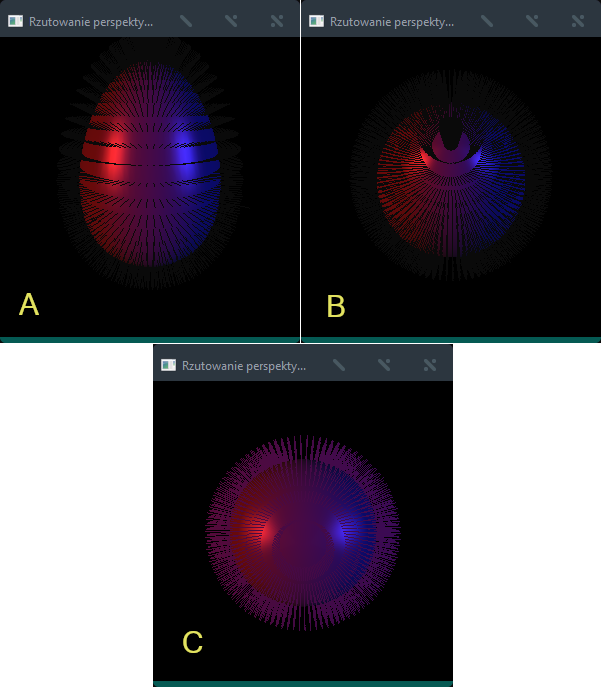
\includegraphics[width=1.0\linewidth]{screen.png}
    \caption{Obiekt oświetlony dwoma źródłami światła (o różnej barwie), obserwowany z boku (A), od góry (B) oraz od spodu (C)}
    \label{fig:screen1}
\end{figure}

\newpage

% ******************************* SPOSTRZEŻENIA I WNIOSKI *******************************

\section{Spostrzeżenia i wnioski}
Teksturowanie powierzchni przy pomocy biblioteki OpenGL okazało się być bardzo złożonym - chociaż nietrudnym w zrozumieniu - zagadnieniem. Największym wyzwaniem okazał się proces debugowania poszarpanej tekstury. Bug ten wynikał z wcześniejszej niewiedzy. Nakładanie tekstury na wierzchołki musi odbywać się przed narysowaniem wierzchołka (podobnie jak z nakładaniem koloru). W innym przypadku oteksturowany zostanie następny w kolejności wierzchołek.

\end{document}